% !TEX root = ../elteikthesis_en.tex
\chapter{User Documentation}
\label{ch:user}

This chapter describes how to set up and use the ELTE IK Assistant.
Two setup paths are provided: a Docker-based zero-configuration path (recommended)
and a manual path for users who prefer to manage dependencies directly.

% ─────────────────────────────────────────────────────────────────────────────
\section{Installation and Configuration}
\label{sec:user-install}

\subsection*{Option A — Docker (recommended)}

Docker Compose orchestrates all services automatically: the Ollama language model
server, the model download, and the FastAPI application.

\begin{enumerate}
    \item Install \textbf{Docker Desktop} (includes Docker Compose) from the official
          Docker website for your operating system.

    \item Clone or download the project repository:
\begin{lstlisting}[language=bash]
git clone https://github.com/borohull/elte_chat.git
cd elte_chat
\end{lstlisting}

    \item Start all services with a single command:
\begin{lstlisting}[language=bash]
docker compose up -d
\end{lstlisting}

    Docker will build the application image, start the Ollama service, and
    automatically pull the \texttt{llama3.2:3b} model on first run.
    This step requires an internet connection and may take several minutes
    depending on download speed.

    \item Once all containers are healthy, open the chat interface at
          \texttt{http://localhost:8000/static/index.html}.

    \item To stop and remove the containers:
\begin{lstlisting}[language=bash]
docker compose down
\end{lstlisting}
\end{enumerate}

\subsection*{Option B — Manual Setup}

For a manual installation without Docker, follow the step-by-step instructions
in Section~\ref{subsec:impl-setup} of the Developer Documentation.

\subsection*{Configuration}

All tunable parameters are defined in \texttt{app/settings.py}.
The most commonly adjusted values are listed in Table~\ref{tab:user-settings}.

\begin{table}[h]
\centering
\begin{tabular}{lll}
\hline
\textbf{Parameter} & \textbf{Default} & \textbf{Description} \\
\hline
\texttt{OLLAMA\_MODEL}    & \texttt{llama3.2:3b}      & Language model served by Ollama \\
\texttt{EMBEDDING\_MODEL} & \texttt{all-MiniLM-L6-v2} & Sentence embedding model \\
\texttt{TOP\_K}           & \texttt{3}                & Chunks retrieved per query \\
\texttt{TEMPERATURE}      & \texttt{0.1}              & Generation temperature \\
\texttt{CHROMA\_PATH}     & \texttt{data/processed/chroma\_db} & Vector store location \\
\hline
\end{tabular}
\caption{Key configuration parameters in \texttt{app/settings.py}}
\label{tab:user-settings}
\end{table}

Changing \texttt{OLLAMA\_MODEL} takes effect on the next server start.
Changing \texttt{EMBEDDING\_MODEL} additionally requires rebuilding the vector
store by re-running notebook \texttt{02\_embedding.ipynb}.

% ─────────────────────────────────────────────────────────────────────────────
\section{Using the Web Interface}
\label{sec:user-web}

Open \texttt{http://localhost:8000/static/index.html} in any modern browser once
the server is running. The interface consists of a left sidebar listing chat
sessions, a central chat panel, and a right sidebar for model selection.

\begin{figure}[H]
    \centering
    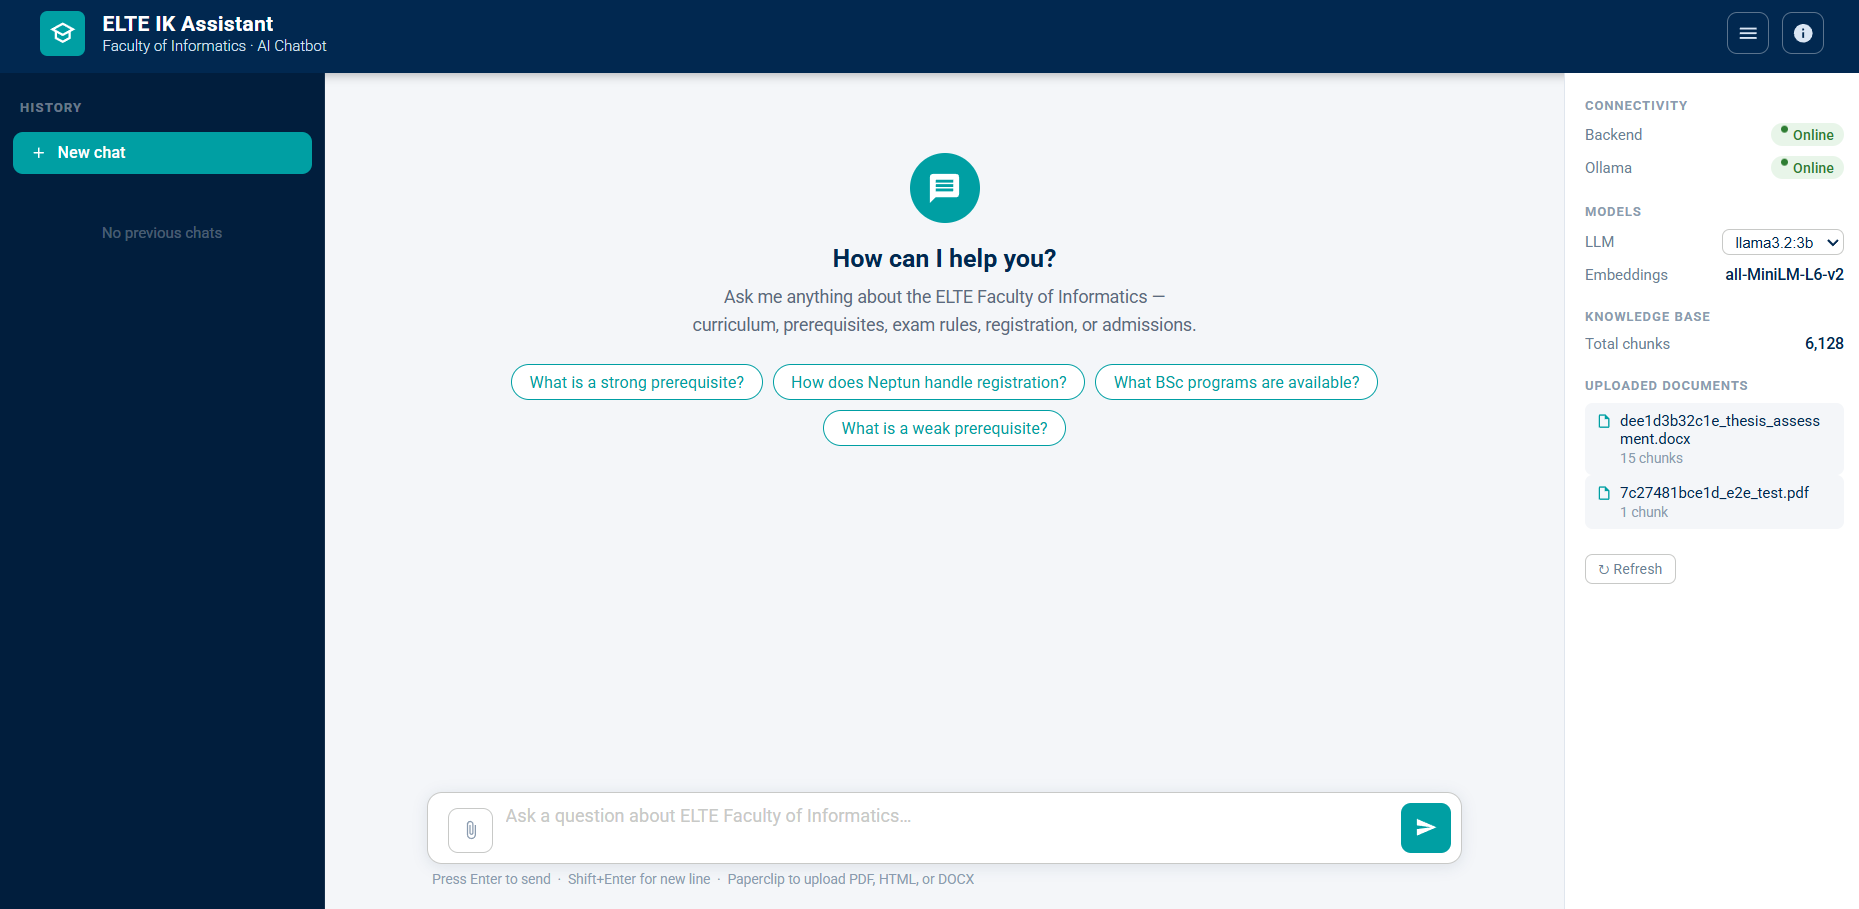
\includegraphics[width=\textwidth]{images/UI.png}
    \caption{The ELTE IK Assistant web interface.}
    \label{fig:ui-screenshot}
\end{figure}

\paragraph{Asking a question.}
Type a question in the input field at the bottom of the chat panel and press
\textbf{Enter} or click the send button. The assistant retrieves relevant document
chunks, constructs a grounded prompt, and returns an answer with source references.
Questions should relate to the ELTE Faculty of Informatics.

\paragraph{Selecting a language model.}
The right sidebar lists all Ollama models available on the machine. Click a model
name to switch for the current session. On a CPU-only machine with 8~GB of RAM,
typical response times are 30--80~seconds per query.

\paragraph{Managing chat sessions.}
Each conversation is stored as a named session. Sessions appear in the left sidebar
and persist across browser refreshes. Click \textbf{New chat} to start a new
conversation, or hover over an existing session and click the \texttimes\ button
to delete it.

\paragraph{Uploading custom documents.}
Users can extend the knowledge base with their own PDF, HTML, or DOCX files.
Click \textbf{Upload document} above the input field, select a file (maximum
20~MB), and wait for the confirmation message. Uploaded documents are chunked,
embedded, and available for retrieval immediately without restarting the server.

% ─────────────────────────────────────────────────────────────────────────────
\section{Using the Command-Line Client}
\label{sec:user-cli}

A lightweight CLI client is provided for scripting and testing without a browser.
The FastAPI server must be running before starting the client:

\begin{lstlisting}[language=bash]
python scripts/chat_cli.py
\end{lstlisting}

Type a question at the \texttt{You:} prompt and press Enter. The client sends the
question to the server and prints the answer. Type \texttt{exit} or press
\texttt{Ctrl+C} to quit.

% ─────────────────────────────────────────────────────────────────────────────
\section{Example Queries}
\label{sec:user-examples}

The following examples illustrate the range of questions the system handles.

\paragraph{Example 1 — Prerequisite query.}
\textit{Question:} ``What is a strong prerequisite and how does it differ from a weak one?''

\textit{Answer:} A strong prerequisite must be passed before a student may register
for the follow-up course. A weak prerequisite allows registration before the
prerequisite is passed, though it is still required for graduation.

\textit{Sources:} \texttt{The\_prerequisites.pdf}

\paragraph{Example 2 — Exam rules.}
\textit{Question:} ``How many times can I retake a failed exam in one semester?''

\textit{Answer:} A student may attempt an exam up to three times per exam period.
If all three attempts are failed, the course must be re-registered in a subsequent
semester.

\textit{Sources:} \texttt{elte\_ik\_regulations.html}

\paragraph{Example 3 — Registration procedure.}
\textit{Question:} ``When does course registration open for the spring semester?''

\textit{Answer:} Course registration for the spring semester typically opens in the
last week of January through the Neptun system. Exact dates are published each year
in the faculty academic calendar.

\textit{Sources:} \texttt{academic\_calendar.html}

\paragraph{Example 4 — Out-of-scope query.}
\textit{Question:} ``What is the capital city of Australia?''

\textit{Answer:} The information needed to answer this question is not available in
the documents I have access to. I can only answer questions related to the ELTE
Faculty of Informatics curriculum, regulations, and procedures.

\textit{Sources:} (none)
